Tras exponer la implementación de los diferentes módulos del sistema, este capítulo detalla su evaluación y la comparación entre las diferentes versiones propuestas.

Con este propósito, inicialmente se explica el sistema de evaluación implementado, tras lo que se exponen los resultados obtenidos y las conclusiones derivadas de dichos resultados. 

\section{Sistema de evaluación}
La solución adoptada sigue los principios establecidos en la Sección \ref{sec:antecedentes_evaluacion}: se evalúa de forma automatizada una serie de métrcias cuantificables (Sección \ref{sec:metricas}) mediante el SDK de LangSmith (Sección \ref{sec:langsmith}) sobre un dataset \textit{ground truth} anotado manualmente (Sección \ref{sec:dataset}) en el dominio del onboarding.

Se ha seleccionado esta metodología de evaluación dada la diversidad de tópicos a los que el sistema debe responder y el conjunto de variaciones implementadas. Frente a una evaluación manual, esta metodología permite ejecutar en pocos minutos las 46 preguntas anotadas, facilitando su ejecución repetida ante cada mejora implementada con una dedicación mínima de recursos.

No obstante, la validación automática del sistema plantea un reto inherente al lenguaje natural: ¿cómo determinar si la respuesta a una pregunta es correcta? Para ello se ha utilizado un LLM como juez, estrategia que consiste en utilizar un agente evaluador cuya función consiste en valorar el resultado obtenido por el agente evaluado.

Para minimizar la tasa de error del juez, se han anotado las respuestas esperadas como listas textuales con los conceptos esenciales a incluir en la respuesta del agente. El agente juez genera una respuesta estructurada con un argumento booleano para cada concepto requerido, indicando si se incluye en la respuesta generada. 

\subsection{Métricas de evaluación}
\label{sec:metricas}
Se han implementado las siguientes métricas para la evaluación de agentes sobre las preguntas anotadas, aplicándose un subconjunto específico de estas según el tipo de agente evaluado:

\paragraph{Precisión del LLM juez} Corresponde al porcentaje de conceptos totales que el LLM juez ha determinado que se incluyen en la respuesta, métrica fundamental para evaluar si la respuesta aborda adecuadamente la pregunta formulada.

Cabe destacar que el juez marcará como incorrecto todo concepto más abstracto que el anotado, aún si conceptualmente el significado es equivalente. Por ejemplo, si se anota que la función del proyecto es proporcionar herramientas de modelos de lenguaje generativos para el equipo de desarrolladores, una respuesta sobre proporcionar herramientas de inteligencia artificial para el equipo sería considerada incorrecta.

\paragraph{Precisión de herramientas} Se comparan las herramientas utilizadas por un agente para responder una pregunta con el listado de herramientas anotado como ideal, lo cual permite identificar comportamientos erróneos cuando el agente no invoca las herramientas necesarias. Se calculan dos métricas posibles:

\begin{itemize}
\item Precisión de herramientas necesarias: indica la cantidad de herramientas necesarias utilizadas, favoreciendo el uso de estas.
\item Precisión de herramientas innecesarias: indica la cantidad de herramientas innecesarias ignoradas, desfavoreciendo el uso de estas.
\end{itemize}

A modo de ejemplo, un agente podría tener 5 herramientas disponibles, de las cuales 2 son necesarias, 2 son innecesarias, y otra no se clasifica en ninguno de los dos grupos, pudiendo ser de utilidad pero no indispensable. Si este llama a 1 necesaria y 2 innecesarias, la precisión necesaria sería de 0.5, mientras que la innecesaria sería de 0.0. La media total sería de 0.25. El uso de la herramienta no clasificada no varía ninguna precisión.

\paragraph{Precisión de alucinación} Los modelos tienden a responder las consultas realizadas aún si no contienen el conocimiento necesario para ello. Para evaluar esto, se han anotado algunas preguntas que son imposibles de responder con la información a la que el agente tiene acceso. Ante la consulta: \texttt{¿Qué flujo de despliegue continuo se utiliza?}, el agente no podrá responder correctamente porque no existe dicho flujo.

Esto es evaluado mediante un agente juez, el cual determina si la respuesta del agente realmente intenta responder a la pregunta o, por el contrario, reconoce que no se dispone de la información suficiente. Esta métrica evalúa, por tanto, el porcentaje de preguntas marcadas como imposibles ante las cuales el sistema se abstiene correctamente de responder.

\paragraph{Precisión de citación} Constituye la cantidad de documentos citados en la respuesta que estaban anotados como necesarios, métrica que permite evaluar el funcionamiento del sistema de citas.

\paragraph{Uso de tokens y costo económico} Las evaluaciones de LangSmith permiten consultar el número de tokens empleados (tanto de entrada como de salida) en las evaluaciones, así como calcular su costo económico según los precios de la API correspondiente. Esta métrica resulta relevante ya que un sistema con menor consumo de tokens representa un sistema con menor redundancia y, por tanto, mayor simplicidad.

\subsection{Implementación de evaluación}
\label{sec:langsmith}
El sistema de evaluación de LangSmith, ilustrado en la Figura \ref{fig:mem_1}, consiste en ejecutar cada ejemplo en el conjunto de datos de forma asíncrona con el agente evaluado. El resultado de cada ejecución se combina con el resultado anotado, y el evaluador correspondiente a cada métrica compara los resultados. Posteriormente, se calcula el promedio de cada métrica para todos los ejemplos de evaluación.

\begin{figure}[h]
\centering
\adjustbox{center=\textwidth}{\includegraphics[width=1\linewidth]{figures/evaluacion.png}}
\caption{Mecanismo de evaluación de agentes}
\label{fig:mem_1}
\end{figure}

Para ello, se utiliza la función \opus{evaluate_agent()} heredada por todos los agentes, la cual define una serie de instancias \opus{BaseEvaluator} que representan los evaluadores a ejecutar. Este diseño permite configurar de forma modular las métricas específicas para cada tipo de agente según sus características particulares. El Listado \ref{lst:evaluate} ilustra dicha función para los agentes especializados.

\begin{lstlisting}[caption={Evaluación de agentes especializados},label={lst:evaluate}]
async def evaluate_agent(self, langsmith_client: Client):
    evaluators = [
        ToolPrecisionEvaluator(self.get_tools_from_run_state),
        JudgeLLMEvaluator(),
        CiteEvaluator()
    ]
    result = await self.call_agent_evaluation(langsmith_client, evaluators)
    return result
\end{lstlisting}

Esta función utiliza internamente las funciones de evaluación de LangSmith mediante \opus{call_agent_evaluation} (Listado \ref{lst:call_evaluation}) para ejecutar todos los ejemplos del conjunto de datos y evaluarlos con las métricas proporcionadas. El conjunto de datos de cada agente va ligado a su nombre y se obtiene mediante el cliente de LangSmith.

\begin{lstlisting}[caption={Llamada a evaluación de agentes},label={lst:call_evaluation}]
async def call_agent_evaluation(self, langsmith_client: Client, 
                               evaluators: List[BaseEvaluator], ...):
    ...
    evaluator_functions = [evaluator.evaluate_metrics for evaluator in evaluators]
    data=langsmith_client.list_examples(dataset_name=dataset_name, splits=splits)
    run_function = self.execute_from_dataset

    results = await aevaluate(
        run_function,
        data=data,
        client=langsmith_client,
        evaluators=evaluator_functions,
        max_concurrency=max_conc,
        experiment_prefix=evaluation_name,
    )
    return results
\end{lstlisting}

El Listado \ref{lst:cite_evaluator} muestra la implementación del evaluador de citas, donde se utilizan el estado de ejecución y el ejemplo anotado para calcular la precisión.

\begin{lstlisting}[caption={Evaluador de citas},label={lst:cite_evaluator}]
class CiteEvaluator(BaseEvaluator):
    async def evaluate(self, run: Run, example: Example) -> EvaluationResults:
        run_state = run.outputs.get("run_state")
        expected_cites = example.outputs.get("cite")
        expected_cites_list = get_list_from_string_comma_separated_values(expected_cites)
        actual_cites = get_cites_from_state_messages(run_state)

        citation_score = get_citation_score(expected_cites_list, actual_cites)
        return EvaluationResults(
            results=[
                EvaluationResult(
                    key="cite_precision",
                    score=StrictFloat(citation_score)
                )
            ]
        )
\end{lstlisting}


\subsection{Dataset ground truth}
\label{sec:dataset}
La captura del conjunto de datos se ha realizado en una hoja de cálculo de Google Drive. Este documento se ha descargado posteriormente en formato de valores separados por coma (CSV) y se ha exportado como conjunto de datos a la plataforma LangSmith.

La captura comprende 46 ejemplos para el agente principal (el sistema completo) y aproximadamente 10 ejemplos para cada agente individual. Para ello se han utilizado las preguntas anotadas en la captura de requisitos, filtrando y modificando en algunos casos las preguntas para ser lo suficientemente específicas como para tener una respuesta exacta, pero a su vez con cierto grado de complejidad que requiera un razonamiento sobre la consulta. Se han utilizado las siguientes consideraciones sobre cada agente:

\begin{itemize}
  \item\textbf{Agente principal: }comprende tres tipos de preguntas según su complejidad: consultas respondibles mediante una única fuente de datos, las que requieren múltiples fuentes, y las que necesitan múltiples fuentes en orden secuencial con dependencias entre ellas. Una pregunta del último tipo es: \texttt{¿Quién ha implementado la funcionalidad de embeddings de Mistral?} 

  \item\textbf{Planificador: }para este agente se ha anotado la respuesta como el plan generado para un ejemplo de ejecución, incluyendo la pregunta y el estado de ejecución actual. Se han identificado tres escenarios: preguntas donde se requiere un solo paso, preguntas donde se requieren varios pasos, y preguntas a medio completar donde se requiere que el agente genere el siguiente paso o decida finalizar el plan. Por ejemplo, en el siguiente ejemplo se ha anotado también un plan a medio completar donde el agente recibe las funcionalidades marcadas por implementar, con el objetivo de que el planificador indique que se deben buscar las incidencias relacionadas en el siguiente paso: \texttt{¿Existe alguna issue para las funcionalidades marcadas en la documentación por implementar?} 
\item\textbf{Orquestador: }este agente se ha evaluado considerando los agentes seleccionados para ejecutar como herramientas. Con tal fin, se han incluido preguntas de todas las temáticas, evaluando qué agentes llamar en cada caso:

\begin{itemize}
\item \textbf{Tareas de agente único: }contempla consultas diseñadas específicamente para cada agente especializado.

\item \textbf{Tareas multi-agente:} las consultas de información general y documentación requieren principalmente el \opus{file_system_agent}, mientras que las de entorno y despliegue combinan este con el \opus{code_agent}. Las preguntas sobre arquitectura del sistema utilizan ambos agentes, y las de gestión del proyecto emplean el \opus{file_system_agent} junto con otros según el contexto específico. Para estándares y prácticas se añade el \opus{confluence_agent} cuando involucran frontend, y las tareas específicas de frontend combinan los agentes \opus{confluence_agent} y \opus{google_drive_agent}.

\end{itemize}
\item\textbf{Agentes sistema de ficheros, Confluence y Google Drive}: en los casos sencillos es necesario únicamente la herramienta de lectura de páginas. En los más desafiantes se requiere de las herramientas de búsqueda: \texttt{¿Cuáles son los colores principales y secundarios de la aplicación?}
\item\textbf{Agente GitLab: }incluye ejemplos donde este debe llamar primero a la herramienta de obtener información sobre los usuarios para posteriormente utilizar esos nombres de usuario como parámetros en otras herramientas. Por ejemplo, en la siguiente consulta el agente deberá buscar cuál es el nombre de usuario de ``Mikel'': \texttt{¿Cuál es el id del último commit de Mikel en 2024?}
\item\textbf{Agente código: }en los casos sencillos los fragmentos relevantes deberían estar incluidos en el prompt de entrada, mientras que en los más complejos debería buscar información adicional: \texttt{¿Puedes mostrarme la jerarquía completa de llamadas para el método invoke\_rag\_with\_repo en ModelTools?}
\end{itemize}

\section{Resultados obtenidos}
En esta sección se presentan los resultados obtenidos mediante el sistema implementado. Inicialmente, se exponen los resultados de evaluación correspondientes a la versión inicial de cada agente, contrastados con una segunda versión mejorada. A continuación se evalúan los distintos sistemas de orquestación desarrollados. Finalmente se analizan las mejoras introducidas en el sistema. Los datos completos de todas las evaluaciones realizadas están públicamente disponibles en el repositorio del proyecto en GitHub para su consulta y reproducibilidad. Dichos datos corresponden a archivos CSV exportados directamente desde la plataforma LangSmith, que incluyen la traza completa de respuestas y los valores de precisión obtenidos para cada métrica.

Cabe destacar que los LLM utilizados no son deterministas: una misma pregunta puede generar respuestas diferentes. Además, al evaluar estas respuestas mediante otro modelo, se introduce una segunda capa de indeterminismo. Esto implica que el sistema presenta una tasa de error variable.

Los resultados mostrados corresponden al promedio de al menos dos ejecuciones. Si bien esto no garantiza certeza absoluta, sí permite afirmar que una evaluación más favorable tiene mayor probabilidad de ser una mejor solución. Esta metodología permite mejorar el sistema de manera objetiva, ya que las mejoras que generen resultados consistentemente superiores en las evaluaciones tienen mayor probabilidad de constituir avances reales.

\subsection{Mejora de versión inicial}
Primero se mejoraron los agentes especializados que presentaron deficiencias en la evaluación inicial, incorporándose posteriormente el prompting few-shot en el orquestador y planificador.

\subsubsection{Agentes especializados}
La Figura \ref{fig:eval_esp} ilustra el rendimiento de los agentes especializados según las métricas de juez, citación y alucinación, así como su gasto promedio por cada ejemplo de ejecución en el dataset.

\begin{figure}[hbtp]
\centering

% Definir estilos comunes para todos los gráficos
\pgfplotsset{
    mybar/.style={
        ylabel=,  
        xlabel=,
        x tick label style={font=\tiny},
        yticklabel style={font=\tiny},
        ymin=0,
        enlarge x limits=0.12,
        ybar=4pt,
        bar width=5pt,
        symbolic x coords={Código, Confluence, S. ficheros, G. Drive, GitLab},
        xtick={Código, Confluence, S. ficheros, G. Drive, GitLab},
        x tick label style={rotate=45, anchor=east, font=\scriptsize},
        width=4.3cm,
        height=4.5cm,
        grid=major,
        grid style={dashed, gray!30},
        tick label style={font=\scriptsize},
        legend style={draw=none},
        scale only axis,
    }
}

% Primera fila con tres gráficos usando minipage
\begin{minipage}{0.32\textwidth}
\centering
\subfloat[LLM juez\label{fig:llm_juez}]{
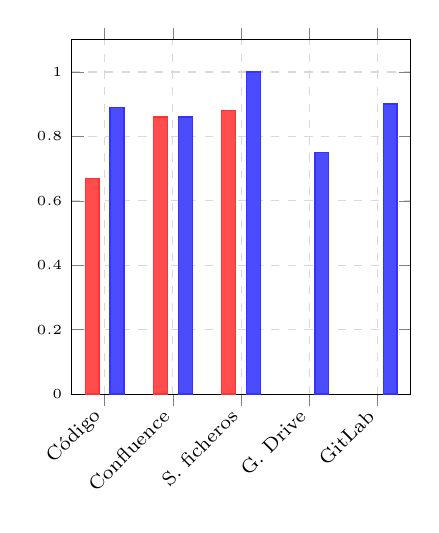
\begin{tikzpicture}
\begin{axis}[
    mybar,
    ymax=1.1,
    ytick={0,0.2,0.4,0.6,0.8,1.0},
]
\addplot[
    fill=red!70,
    draw=red!80,
    line width=0.5pt
] coordinates {
    (Código, 0.67)
    (Confluence, 0.86)
    (S. ficheros, 0.88)
    (G. Drive, nan)
    (GitLab, nan)
};
\addplot[
    fill=blue!70,
    draw=blue!80,
    line width=0.5pt
] coordinates {
    (Código, 0.89)
    (Confluence, 0.86)
    (S. ficheros, 1.0)
    (G. Drive, 0.75)
    (GitLab, 0.9)
};
\end{axis}
\end{tikzpicture}
}
\end{minipage}
\begin{minipage}{0.32\textwidth}
\centering
\subfloat[Precisión citación\label{fig:precision_citas}]{
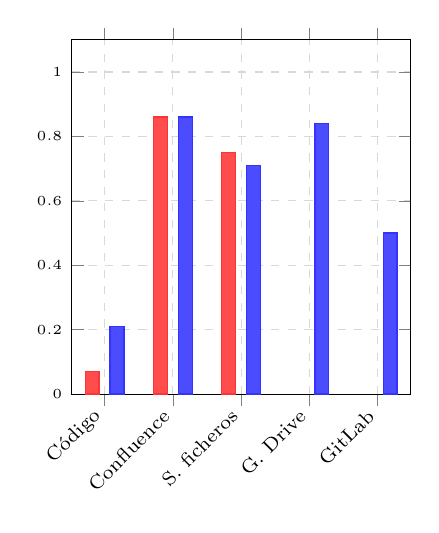
\begin{tikzpicture}
\begin{axis}[
    mybar,
    ymax=1.1,
    ytick={0,0.2,0.4,0.6,0.8,1.0},
]
\addplot[
    fill=red!70,
    draw=red!80,
    line width=0.5pt
] coordinates {
    (Código, 0.07)
    (Confluence, 0.86)
    (S. ficheros, 0.75)
    (G. Drive, nan)
    (GitLab, nan)
};
\addplot[
    fill=blue!70,
    draw=blue!80,
    line width=0.5pt
] coordinates {
    (Código, 0.21)
    (Confluence, 0.86)
    (S. ficheros, 0.71)
    (G. Drive, 0.84)
    (GitLab, 0.5)
};
\end{axis}
\end{tikzpicture}
}
\end{minipage}
\begin{minipage}{0.32\textwidth}
\centering
\subfloat[Precisión de herramientas\label{fig:precision_herramientas}]{
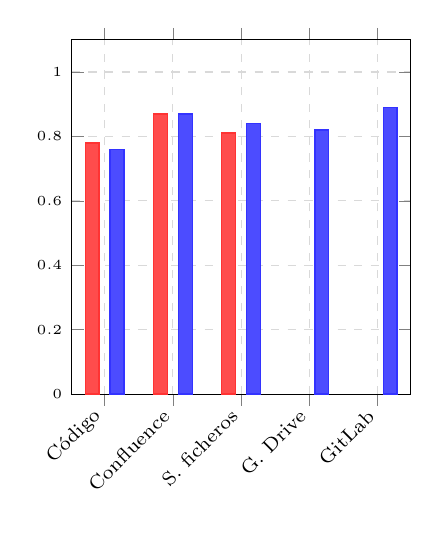
\begin{tikzpicture}
\begin{axis}[
    mybar,
    ymax=1.1,
    ytick={0,0.2,0.4,0.6,0.8,1.0},
]
\addplot[
    fill=red!70,
    draw=red!80,
    line width=0.5pt
] coordinates {
    (Código, 0.78)
    (Confluence, 0.87)
    (S. ficheros, 0.81)
    (G. Drive, nan)
    (GitLab, nan)
};
\addplot[
    fill=blue!70,
    draw=blue!80,
    line width=0.5pt
] coordinates {
    (Código, 0.76)
    (Confluence, 0.87)
    (S. ficheros, 0.84)
    (G. Drive, 0.82)
    (GitLab, 0.89)
};
\end{axis}
\end{tikzpicture}
}
\end{minipage}

\vspace{0.2cm}

% Segunda fila con dos gráficos centrados
\begin{minipage}{0.32\textwidth}
\centering
\subfloat[Alucinación (más es mejor)\label{fig:halucinacion}]{
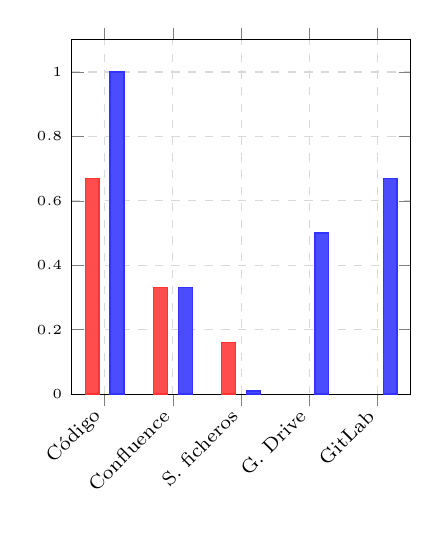
\begin{tikzpicture}
\begin{axis}[
    mybar,
    ymax=1.1,
    ytick={0,0.2,0.4,0.6,0.8,1.0},
]
\addplot[
    fill=red!70,
    draw=red!80,
    line width=0.5pt
] coordinates {
    (Código, 0.67)
    (Confluence, 0.33)
    (S. ficheros, 0.16)
    (G. Drive, nan)
    (GitLab, nan)
};
\addplot[
    fill=blue!70,
    draw=blue!80,
    line width=0.5pt
] coordinates {
    (Código, 1.0)
    (Confluence, 0.33)
    (S. ficheros, 0.01)
    (G. Drive, 0.5)
    (GitLab, 0.67)
};
\end{axis}
\end{tikzpicture}
}
\end{minipage}
\hspace{0.05\textwidth}
\begin{minipage}{0.32\textwidth}
\centering
\subfloat[Tokens por ejecución (millares)\label{fig:tokens}]{
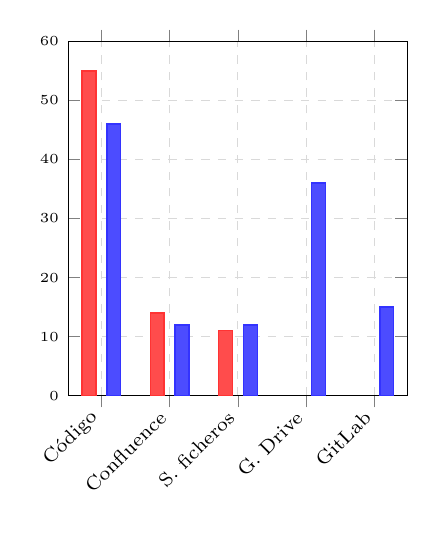
\begin{tikzpicture}
\begin{axis}[
    mybar,
    ymax=60,
    ytick={0,10,20,30,40,50,60},  % Para el gráfico de tokens
]
\addplot[
    fill=red!70,
    draw=red!80,
    line width=0.5pt
] coordinates {
    (Código, 55)
    (Confluence, 14)
    (S. ficheros, 11)
    (G. Drive, nan)
    (GitLab, nan)
};
\addplot[
    fill=blue!70,
    draw=blue!80,
    line width=0.5pt
] coordinates {
    (Código, 46)
    (Confluence, 12)
    (S. ficheros, 12)
    (G. Drive, 36)
    (GitLab, 15)
};
\end{axis}
\end{tikzpicture}
}
\end{minipage}

% Leyenda global centrada (simplificada)
\vspace{-0.2cm} % Justo antes del bloque de leyenda
\begin{center}

\begin{tikzpicture}
    \draw[fill=red!70,draw=red!80,line width=0.5pt] (0,0) rectangle (0.4,-0.25);
    \node[right] at (0.5,-0.125) {Inicial};
    \draw[fill=blue!70,draw=blue!80,line width=0.5pt] (2,0) rectangle (2.4,-0.25);
    \node[right] at (2.5,-0.125) {Mejorado};
\end{tikzpicture}
\end{center}

\caption{Comparación de métricas entre versión inicial y mejorada de agentes especialistas}
\label{fig:eval_esp}
\end{figure}
\vspace{-0.2cm} 

\paragraph{Agente de código}Este presentó un gasto considerablemente superior debido a las múltiples consultas RAG realizadas para una misma pregunta. Se ajustó el prompt y la cantidad de fragmentos extraídos, reduciendo así el coste asociado a ejecuciones prolongadas.

\paragraph{Agente Confluence} Se identificó que la tarea de este agente consistía invariablemente en elegir qué fichero leer y responder basándose en su contenido. Se incorporó el enfoque de prompt caching, ya que al limitarse exclusivamente a leer y responder, el acceso directo a todos los documentos podría reducir los errores derivados de no leer los documentos necesarios. Aunque la precisión en todas las métricas resultó similar, este enfoque redujo el consumo de tokens y el gasto económico.

\paragraph{Agente sistema de ficheros}
Al requerir la selección entre múltiples ficheros, cuyos nombres en ciertas situaciones no describían adecuadamente todo su contenido, este agente presentaba dificultades para identificar los documentos necesarios. Por ello, la mejora implementada consistió en la inclusión de la herramienta RAG. Cuando existe incertidumbre sobre cuál fichero leer, esta herramienta proporciona varios fragmentos relacionados junto al nombre del fichero, facilitando así la localización de la información requerida.

\subsubsection{Planificador y orquestador}
El principal problema identificado en estos agentes radicaba en su incumplimiento del comportamiento esperado. Mientras que el agente planificador tendía a incluir pasos innecesarios, el agente orquestador invocaba un número excesivo de agentes especializados. La mejora implementada consistió en incorporar varios ejemplos del comportamiento esperado en los prompts correspondientes.

La Figura \ref{fig:eval_fewshots} ilustra la comparación del agente planificador y orquestador tras incorporar el prompting few-shot. Los resultados muestran una mejora considerable en el rendimiento de ambos agentes.


\begin{figure}[hbtp]
\centering

% Primera fila con tres gráficos usando minipage
\begin{minipage}{0.32\textwidth}
\centering
\subfloat[LLM juez\label{fig:llm_judge_agentes}]{
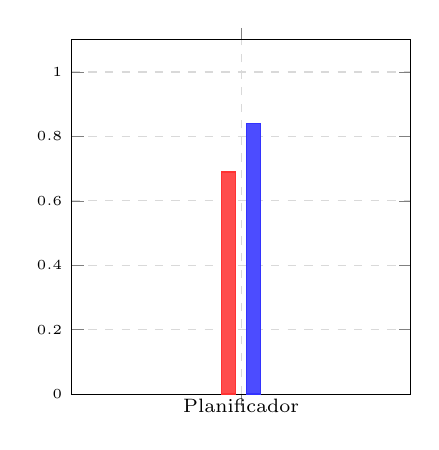
\begin{tikzpicture}
\begin{axis}[
    ylabel=,  
    xlabel=,
    ymin=0,
    ymax=1.1,
    ytick={0,0.2,0.4,0.6,0.8,1.0},
    enlarge x limits=0.8,
    ybar=4pt,
    bar width=5pt,
    symbolic x coords={Planificador},
    xtick={Planificador},
    x tick label style={rotate=0, anchor=center, font=\scriptsize},
    yticklabel style={font=\tiny},
    width=4.3cm,
    height=4.5cm,
    grid=major,
    grid style={dashed, gray!30},
    tick label style={font=\scriptsize},
    scale only axis,
]
\addplot[
    fill=red!70,
    draw=red!80,
    line width=0.5pt
] coordinates {
    (Planificador, 0.69)
};
\addplot[
    fill=blue!70,
    draw=blue!80,
    line width=0.5pt
] coordinates {
    (Planificador, 0.84)
};
\end{axis}
\end{tikzpicture}
}
\end{minipage}
\begin{minipage}{0.32\textwidth}
\centering
\subfloat[Precisión herramientas\label{fig:tool_precision_agentes}]{
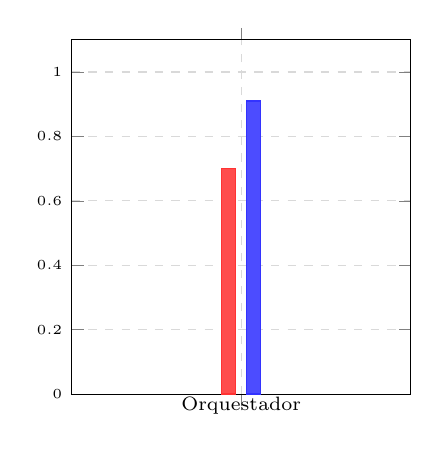
\begin{tikzpicture}
\begin{axis}[
    ylabel=,  
    xlabel=,
    ymin=0,
    ymax=1.1,
    ytick={0,0.2,0.4,0.6,0.8,1.0},
    enlarge x limits=0.8,
    ybar=4pt,
    bar width=5pt,
    symbolic x coords={Orquestador},
    xtick={Orquestador},
    x tick label style={rotate=0, anchor=center, font=\scriptsize},
    yticklabel style={font=\tiny},
    width=4.3cm,
    height=4.5cm,
    grid=major,
    grid style={dashed, gray!30},
    tick label style={font=\scriptsize},
    scale only axis,
]
\addplot[
    fill=red!70,
    draw=red!80,
    line width=0.5pt
] coordinates {
    (Orquestador, 0.70)
};
\addplot[
    fill=blue!70,
    draw=blue!80,
    line width=0.5pt
] coordinates {
    (Orquestador, 0.91)
};
\end{axis}
\end{tikzpicture}
}
\end{minipage}
\begin{minipage}{0.32\textwidth}
\centering
\subfloat[Alucinación (más es mejor)\label{fig:alucinacion_agentes}]{
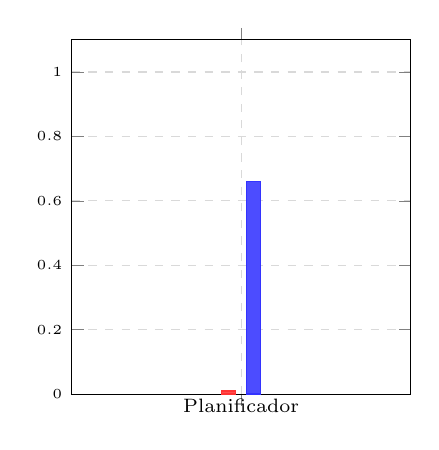
\begin{tikzpicture}
\begin{axis}[
    ylabel=,  
    xlabel=,
    ymin=0,
    ymax=1.1,
    ytick={0,0.2,0.4,0.6,0.8, 1.0},
    enlarge x limits=0.8,
    ybar=4pt,
    bar width=5pt,
    symbolic x coords={Planificador},
    xtick={Planificador},
    x tick label style={rotate=0, anchor=center, font=\scriptsize},
    yticklabel style={font=\tiny},
    width=4.3cm,
    height=4.5cm,
    grid=major,
    grid style={dashed, gray!30},
    tick label style={font=\scriptsize},
    scale only axis,
]
\addplot[
    fill=red!70,
    draw=red!80,
    line width=0.5pt
] coordinates {
    (Planificador, 0.01)
};
\addplot[
    fill=blue!70,
    draw=blue!80,
    line width=0.5pt
] coordinates {
    (Planificador, 0.66)
};
\end{axis}
\end{tikzpicture}
}
\end{minipage}

% Leyenda global centrada
\vspace{-0.2cm}
\begin{center}

\begin{tikzpicture}
    \draw[fill=red!70,draw=red!80,line width=0.5pt] (0,0) rectangle (0.4,-0.25);
    \node[right] at (0.5,-0.125) {Inicial};
    \draw[fill=blue!70,draw=blue!80,line width=0.5pt] (2,0) rectangle (2.4,-0.25);
    \node[right] at (2.5,-0.125) {Mejorado};
\end{tikzpicture}
\end{center}

\caption{Evaluación de agentes orquestador y planificador antes y después de prompting few-shot}
\label{fig:eval_fewshots}
\end{figure}
\vspace{-0.2cm}

\subsection{Variaciones de orquestación}
\label{sec:eval_orch}
Esta evaluación (Figura \ref{fig:eval_orch}) compara los diferentes enfoques de orquestación: planificación dividida, planificación unificada, el sistema sin planificación y el sistema adaptativo. Adicionalmente, se incluye la evaluación del sistema inicial (planificación dividida previa a las mejoras implementadas en la sección anterior).

Los resultados muestran que las mejoras implementadas incrementaron significativamente el rendimiento del sistema mejorado en comparación con la versión inicial. El prompting few-shot en el orquestador y planificador redujo la cantidad de agentes utilizados, optimizando notablemente el costo total.

\begin{figure}[hbtp]
\centering

% Primera fila con dos gráficos usando minipage
\begin{minipage}{0.48\textwidth}
\centering
\subfloat[LLM juez\label{fig:llm_judge_sistemas}]{
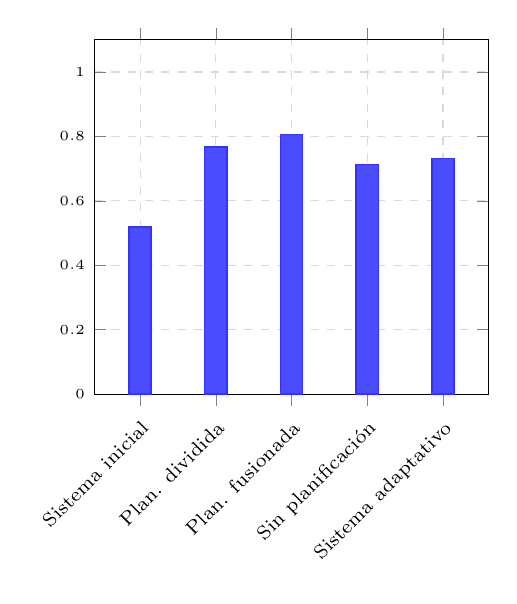
\begin{tikzpicture}
\begin{axis}[
    ylabel=,  
    xlabel=,
    ymin=0,
    ymax=1.1,
    ytick={0,0.2,0.4,0.6,0.8,1.0},
    enlarge x limits=0.15,
    ybar=4pt,
    bar width=8pt,
    symbolic x coords={Sistema inicial, Plan. dividida, Plan. fusionada, Sin planificación, Sistema adaptativo},
    xtick={Sistema inicial, Plan. dividida, Plan. fusionada, Sin planificación, Sistema adaptativo},
    x tick label style={rotate=45, anchor=north east, font=\scriptsize},
    yticklabel style={font=\tiny},
    width=5cm,
    height=4.5cm,
    grid=major,
    grid style={dashed, gray!30},
    tick label style={font=\scriptsize},
    scale only axis,
]
\addplot[
    fill=blue!70,
    draw=blue!80,
    line width=0.5pt
] coordinates {
    (Sistema inicial, 0.5183)
    (Plan. dividida, 0.7665)
    (Plan. fusionada, 0.805)
    (Sin planificación, 0.7126)
    (Sistema adaptativo, 0.7307)
};
\end{axis}
\end{tikzpicture}
}
\end{minipage}
\begin{minipage}{0.48\textwidth}
\centering
\subfloat[Costo total de tokens (millones)\label{fig:token_cost_sistemas}]{
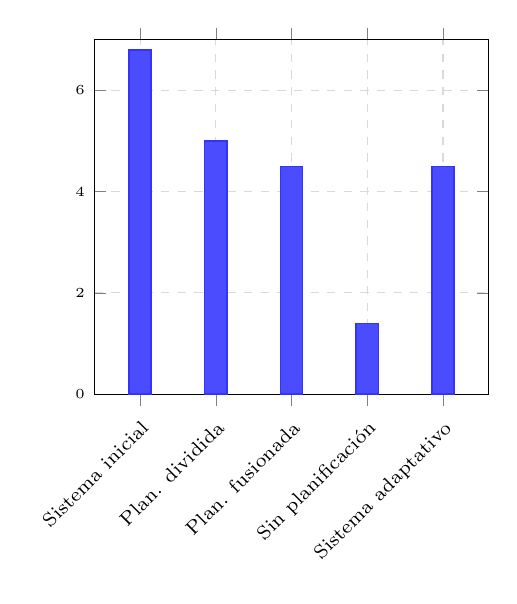
\begin{tikzpicture}
\begin{axis}[
    ylabel=,  
    xlabel=,
    ymin=0,
    ymax=7,
    ytick={0,2,4,6,8},
    enlarge x limits=0.15,
    ybar=4pt,
    bar width=8pt,
    symbolic x coords={Sistema inicial, Plan. dividida, Plan. fusionada, Sin planificación, Sistema adaptativo},
    xtick={Sistema inicial, Plan. dividida, Plan. fusionada, Sin planificación, Sistema adaptativo},
    x tick label style={rotate=45, anchor=north east, font=\scriptsize},
    yticklabel style={font=\tiny},
    width=5cm,
    height=4.5cm,
    grid=major,
    grid style={dashed, gray!30},
    tick label style={font=\scriptsize},
    scale only axis,
]
\addplot[
    fill=blue!70,
    draw=blue!80,
    line width=0.5pt
] coordinates {
    (Sistema inicial, 6.8)
    (Plan. dividida, 5.0)
    (Plan. fusionada, 4.5)
    (Sin planificación, 1.4)
    (Sistema adaptativo, 4.5)
};
\end{axis}
\end{tikzpicture}
}
\end{minipage}

\caption{Comparación de rendimiento y costo entre diferentes variaciones de orquestación}
\label{fig:eval_orch}
\end{figure}
\vspace{-0.2cm}

En cuanto a la planificación, los resultados confirman que esta etapa mejora en ambos casos el sistema. Específicamente, la planificación unificada supera a la dividida. Esto indica que, en este caso de uso, la división lógica del paso de planificación no resulta eficiente, siendo preferible que el agente planificador disponga directamente de la máxima información posible para fundamentar su plan.

Finalmente, los resultados del enfoque adaptativo no cumplieron las expectativas. Aunque el rendimiento se situó en el rango esperado —superior al sistema sin planificación pero inferior a la planificación unificada— y el coste resultó menor que la planificación tradicional (al no emplear modelos razonadores pese al uso similar de tokens), la mejora económica resultó mínima mientras que la pérdida de rendimiento fue considerable. Estos resultados indican que el enfoque adaptativo no es adecuado para este caso de uso, siendo la planificación unificada la opción más eficiente.

\subsection{Integración de memoria}
Para evaluar este componente, se dividió el dataset del agente principal en un conjunto de entrenamiento (80\%) y de evaluación (20\%). Se analizó si las memorias acumuladas sobre el conjunto de entrenamiento mejoran el rendimiento en el conjunto de evaluación, ejecutando el sistema secuencialmente sobre ambos conjuntos y comparando el rendimiento con y sin memoria.

La Figura \ref{fig:mem_train} muestra que incluir memorias de entrenamiento mejoró la precisión en el conjunto de evaluación respecto al sistema sin memoria. Sin embargo, la Figura \ref{fig:mem_test} presenta resultados menos prometedores al evaluar repetidamente el conjunto de evaluación añadiendo memorias de los mismos ejemplos de evaluación. Esto indica que, en este caso, la memoria funciona mejor como información adicional que como memoria caché.

\begin{figure}[hbtp]
\centering
% Primera fila con dos gráficos usando minipage
\begin{minipage}{0.48\textwidth}
\centering
\subfloat[Evaluación con memorias de entrenamiento sobre conjunto de evaluación\label{fig:memoria_comparacion}]{
\label{fig:mem_train}
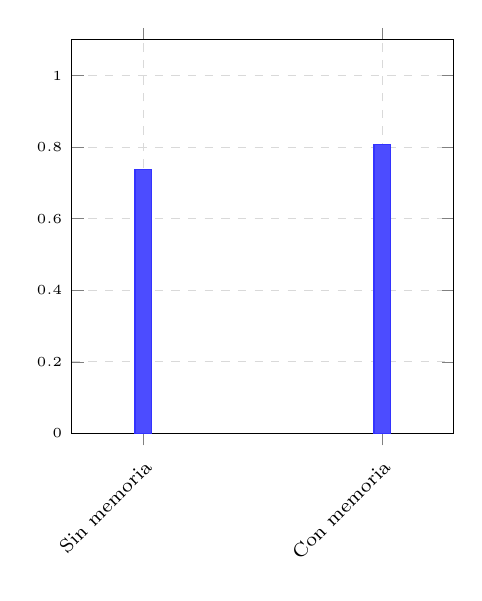
\begin{tikzpicture}
\begin{axis}[
    ylabel=,  
    xlabel=,
    ymin=0,
    ymax=1.1,
    ytick={0,0.2,0.4,0.6,0.8,1.0},
    height=5cm,
    enlarge x limits=0.3,
    ybar=2pt,
    bar width=6pt,
    symbolic x coords={Sin memoria, Con memoria},
    xtick={Sin memoria, Con memoria},
    x tick label style={rotate=45, anchor=north east, font=\scriptsize},
    yticklabel style={font=\tiny},
    grid=major,
    grid style={dashed, gray!30},
    tick label style={font=\scriptsize},
    scale only axis,
    width=4.85cm,
]
\addplot[
    fill=blue!70,
    draw=blue!80,
    line width=0.5pt
] coordinates {
    (Sin memoria, 0.7377)
    (Con memoria, 0.8066)
};
\end{axis}
\end{tikzpicture}
}
\end{minipage}
\begin{minipage}{0.44\textwidth}
\centering
\subfloat[Evaluación con memorias de evaluación sobre conjunto de evaluación\label{fig:evolucion_trials}]{
\label{fig:mem_test}
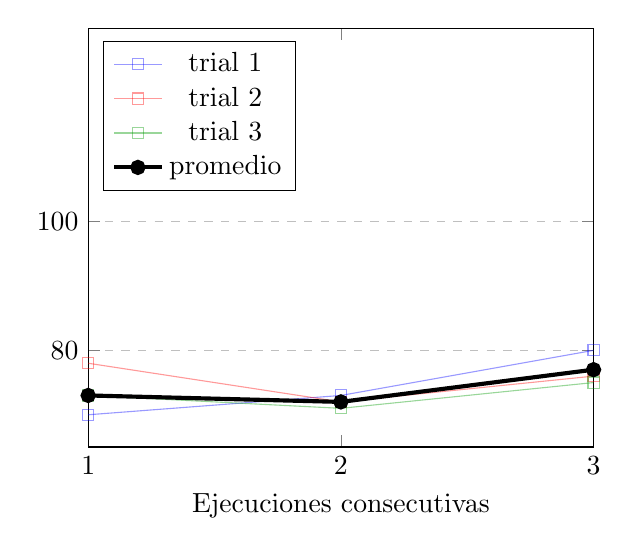
\begin{tikzpicture}
\begin{axis}[
    title={},
    xlabel={Ejecuciones consecutivas},
    ylabel={},
    xmin=1, xmax=3,
    ymin=65, ymax=130,
    xtick={1, 2, 3},
    ytick={0,20,40,60,80,100},
    legend pos=north west,
    ymajorgrids=true,
    grid style=dashed,
    width=8cm,
]
% gráfico original trial 1
\addplot[
    color=blue,
    mark=square,
    opacity=0.4,
    ]
    coordinates {
    (1, 70)(2, 73)(3, 80) 
    };
% trial 2 
\addplot[
    color=red,
    mark=square,
    opacity=0.4,
    ]
    coordinates {
      (1, 78)(2, 72)(3, 76)
    };
% trial 3 
\addplot[
    color=green!60!black,
    mark=square,
    opacity=0.4,
    ]
    coordinates {
      (1, 73)(2, 71)(3, 75)
    };
% línea promedio
\addplot[
    color=black,
    mark=*,
    line width=1.5pt,
    ]
    coordinates {
      (1, 73)(2, 72)(3, 77)
    };
\legend{trial 1, trial 2, trial 3, promedio}
\end{axis}
\end{tikzpicture}
}
\end{minipage}
\caption{Resultados de evaluación para el sistema con y sin memoria}
\label{fig:memoria_evolucion}
\end{figure}
